\section{Twisting Bezier Splines}
\label{Chapter:SplineModelling}

    \subsection{The need of twisting bezier splines}
    Conventional bezier curves are commonly used to define outline fonts [cite] and digital calligraphy [cite] due to their ability to accurately trace [cite] the outline of scripts written with and without a broad edge tool [cite]. These curves can be easily manipulated [cite] and rendered [cite] on a computer screen as well as they can be printed on paper. However, in light of the underlaying problem, and in order to preserve the essence of artistic norms [cite], it is desired that a script is written using a conventional broad-edge tool by a robotic manipulator [cite] in a similar fashion to a human artist. Separate techniques [cite] are needed to convert output of the outline or pitch curve functions to a format that a robot can directly use for the desired tool movement. Even though many of these techniques [cite] can promise accurate tracing, none of them can promise that the robot will use the exact tool movement of a human agent.

    In most literal terms, beizer spline curves are sets of decimal values that define the graphical shape of certain mathematical functions [cite]. The input of these functions contains two dimensional points located in the frame of reference of the screen on which they are created and work as handles to control the shape of the curve using a screen pointer. A user can physically relocate these curvature handles on the computer screen and the shape of the resulting spline will follow. The output of these mathematical functions is absolutely repeatable and can be linearly scaled to any units. Usually, a curve is made of up a lot of such lines each with its own set of input coefficients. Although these individual functions are continuous, there output can easily be discretized as closed paths made up of closely located two dimensional points with controllable resolution [cite]. This is exactly the kind of information required by most of computer graphics and printing drivers to render an output.

    Now, as effective as the bezier curves are for screen and paper printing, they still cannot tell how a physical tool should move on a piece of paper to create the desired output. The splines are just organic shaped paths with no thickness. One of the ways to convert them into ink-mark, is to interpret them as the pitch line for a thick round tool tip. This technique is used by plotters [cite] and some hand writing replicators [cite] to produce a written script. However, only a few fonts [cite] can be replicated by this technique. The other technique is to fill the glyph by moving the tool continuously on a path computed by algorithms such as those used by CAD tools [cite] to fill in (or cut) the area contained by the outline of the glyph using a thick round tip tool. The later can produce outputs that looks similar to broad-edge calligraphy but will still not be the same due to the visible tool paths that are not expected when using an actual broad edge tool.

%    Conventionally, image processing is being used [cite] to extract data that can be used to create machine data for calligraphy. We, however, propose a difference; no matter how strong and robust image processing gets, we maintain that there is no alternative to the minor details only a real artist can observe and recreate. So a solution is needed that fulfils the technical needs as well as the artistic demands. One can virtually draw any kind of shape that can be represented on a two dimensional surface using the conventional bezier splines but it is not very intuitive to accurately reproduce the output of a broad-edge tool.

    On the other hand, twisting bezier splines, instead of working as outline curves, directly record the pitch line of a twisting broad-edge tool stroke along-with the twist information and recreate the live result to the artist who can than morph the spline in a convenient way as normal splines. Their usage is just as intuitive as the conventional bezier splines and will be demonstrated in the next sections, and the information they contain can not only be used to render the script back on the screen or a photo printer, but also be directly considered as machine data for robotic manipulators.

    In contrast to normal bezier splines, twisting bezier splines not only trace the pitch lines of all the strokes but also the twist of the tool independent of the curvature. This is done by introducing another input to the curve function that we call the ``rotation'' or ``twist'' handle. Just like the curvature handles represent the function inputs responsible to define the curvature of the pitch line which is in fact a normal spline, the rotation handles represent the inputs that control the twist of the simulated broad-edge tool. Just like conventional bezier splines, functions of the twisting bezier splines can also be discretized and converted into a list of two dimensional list of points; a closed path to emulate the ink-mark of the broad edge tool. As was the case with normal splines, this is exactly the kind of data needed by the computer display drivers.

    Interestingly, although the twisting splines originate on a computer screen, they are still nearer to the machine than they are to computer graphics data. To compute the list of the points needed to create a filled path that represents the ink-mark, a broad edge tool is emulated to be moving on the rotating spline with the twist also controlled by the spline. In actuality, the emulated tool is replaced by a real tool that can be mounted on a robotic manipulator. The spline directly controls the position and twist of the tip of a tool which can directly be translated into machine movement codes. The rest of the process for painting involves inverse kinematics [cite] and is already handled by the robot controller.

    \subsection{Mathematical Model of a Twisting Bezier Spline}
    \subsubsection{The Conventional Bezier Spline}
         We first describe conventional bezier splines. Figure \ref{Fig:BezierSplines} illustrates different aspects of a spline path composed of several sub curves. Each curve section is only partly independent of the other. Figure \ref{Fig:BezierSplines} (a) shows how individual splines combine to form a bigger spline path. These sections are labeled $1$ through $5$. Figure \ref{Fig:BezierSplines} (b) shows anchors and curvature handles of each part of the path. For instance, Figure \ref{Fig:BezierSplines} (c) extracts and highlights section $4$ and shows anchor points $A$ and $B$ that control this section. Each anchor has two handles referenced from its position. For example, anchor $A$ has two handles, $H_1$ and $H_2$, connected through a straight line passing through the parent anchor and referenced from the parent anchor. Overall, handles $H_1$, $H_2$, $H_3$ and $H_4$ are attached to the two anchors that control this section, however in addition to the anchors, only $H_2$, $H_3$ are directly responsible to control the curvature of this section. It must be noted here that although the lengths of segments $\overline{AH_2}$ and $\overline{BH_3}$ are not connected to the lengths of segments $\overline{AH_1}$ and $\overline{BH_4}$ respectively, the positions of handles $H_2$ and $H_3$ are also influenced by $H1$ and $H4$. These handles control the curvature of the neighboring sections $3$ and $5$ and thus indirectly influence the shape of section $4$ as well. This is how each section is only partly independent and connected to neighbouring sections.



        \begin{figure}[!t]
            \centering
            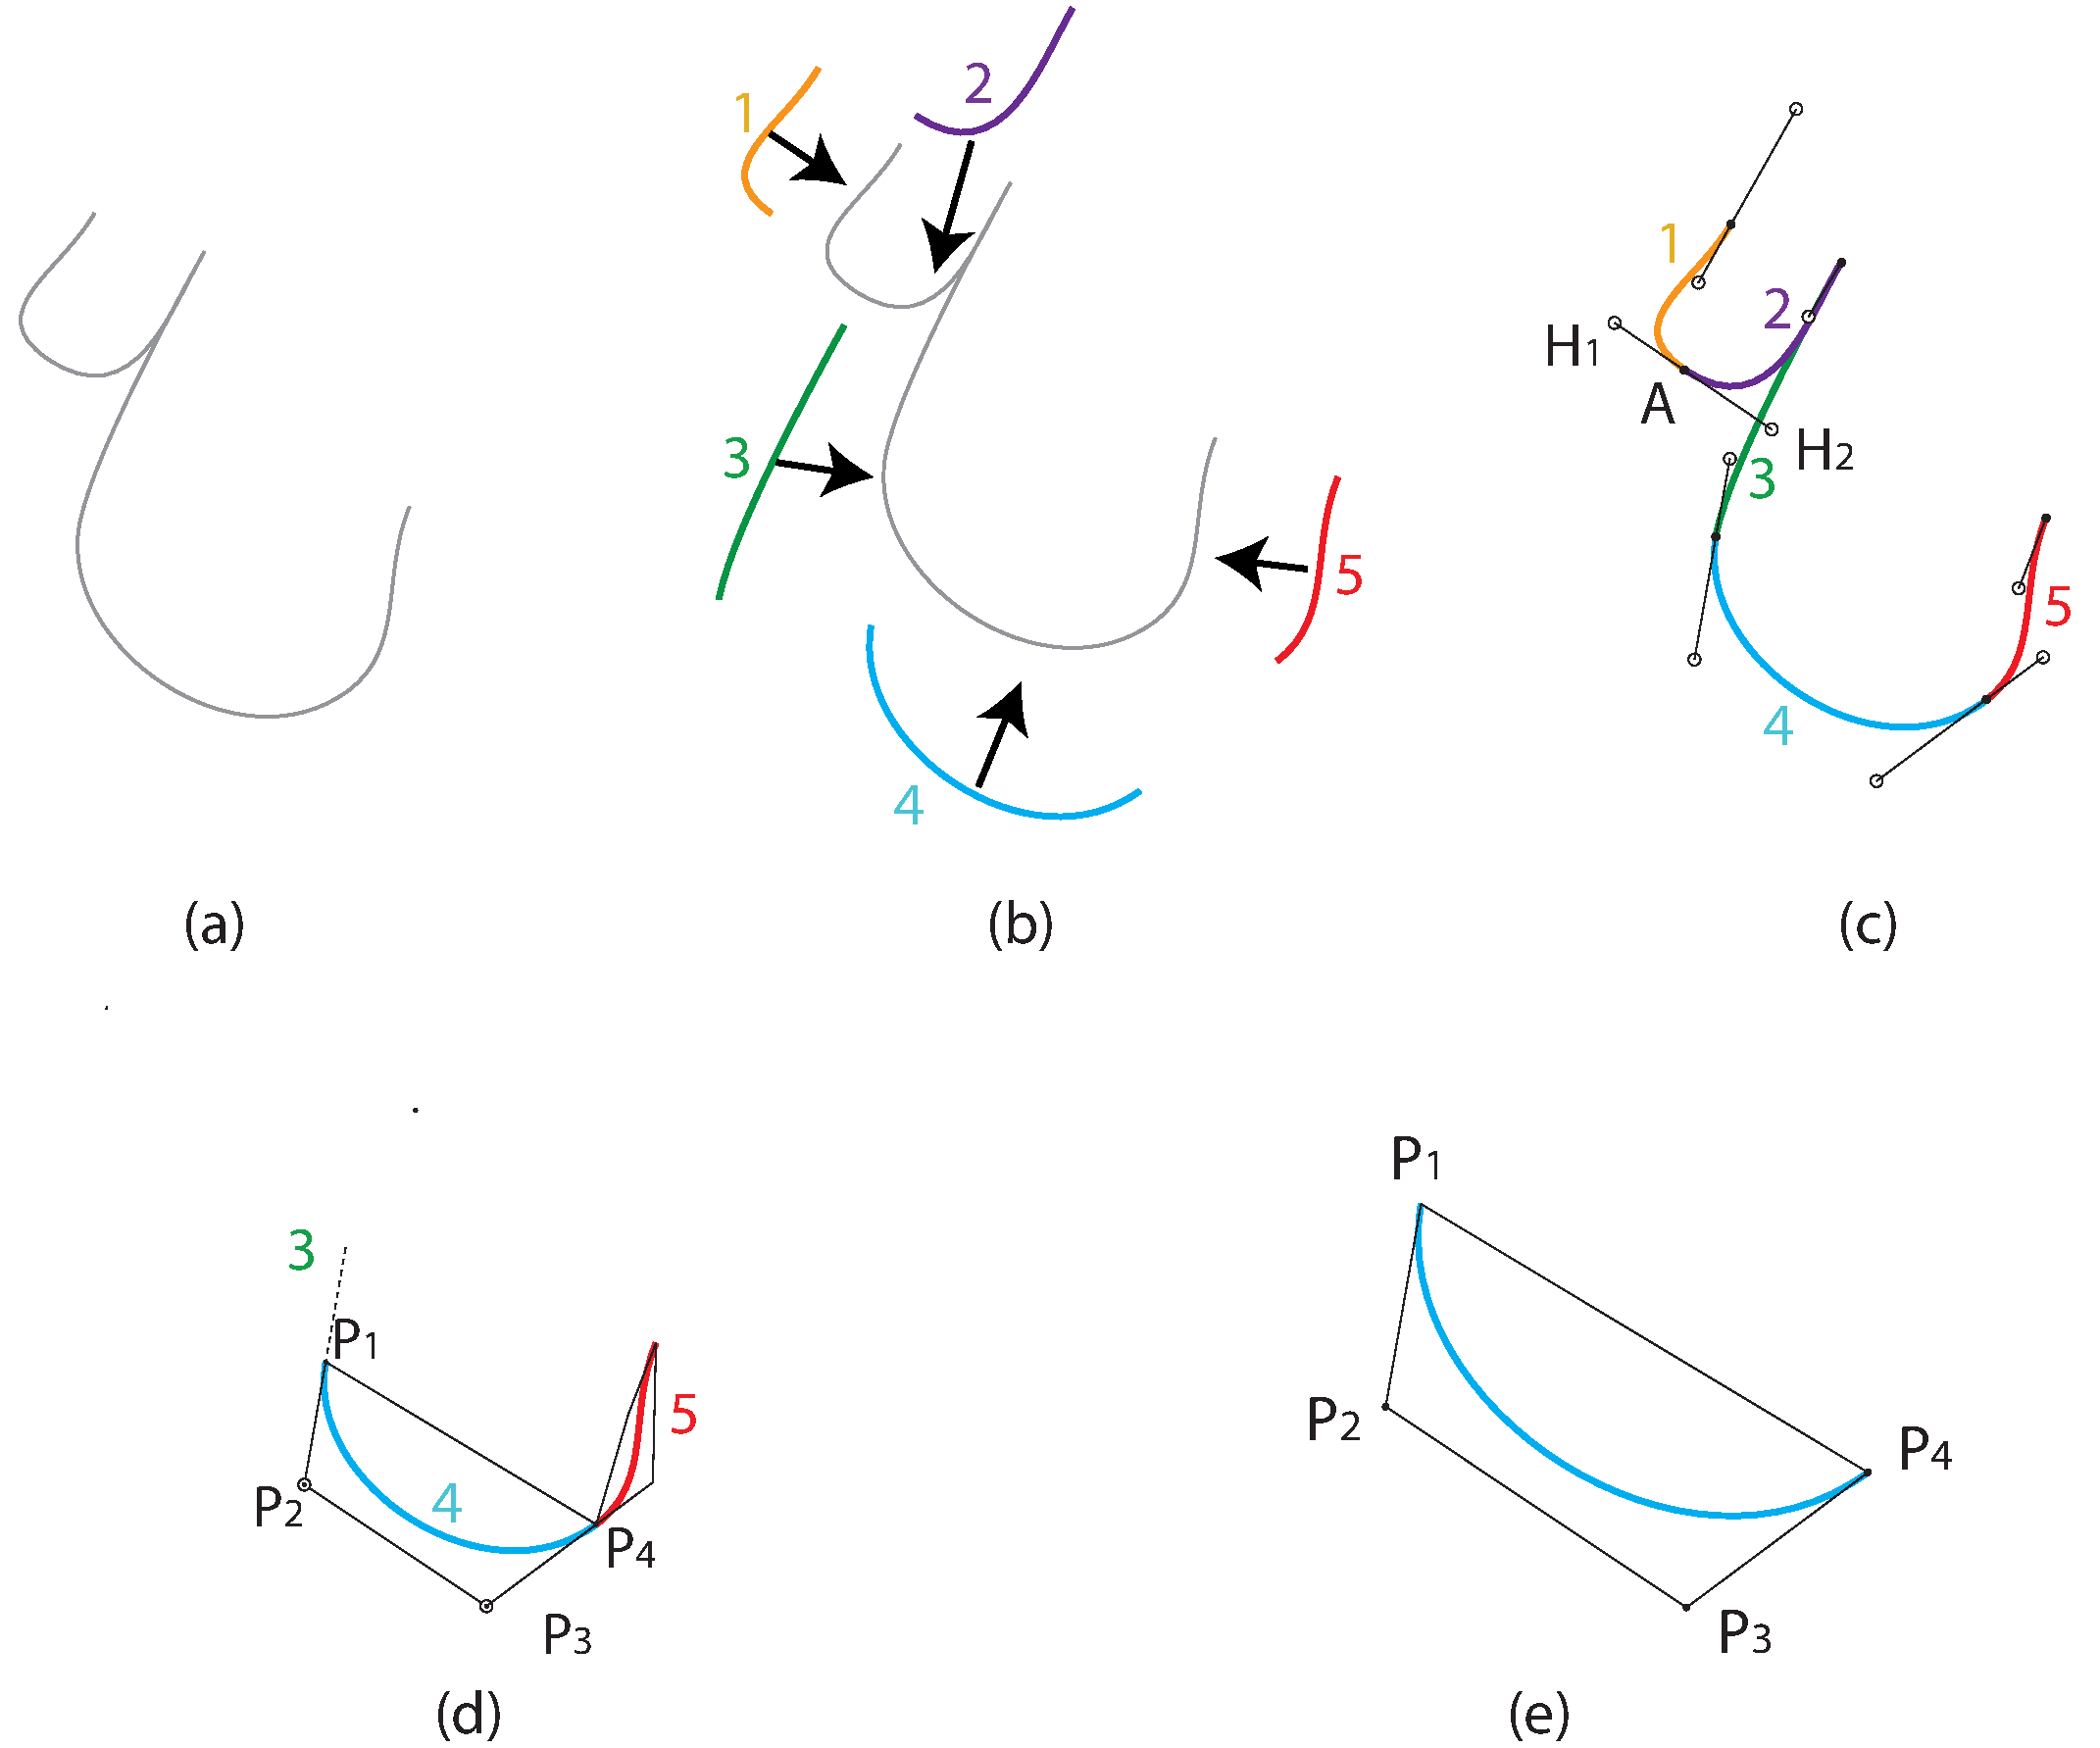
\includegraphics[width=2.5in]{../Images/BezierSplineCurve.pdf}
            \caption{The figure first illustrates how a spline is constructed and is transformed to a twisting bezier spline. (a) An exploded view of a bezier spline path that show the individual splines that compose the parent path. (b) Control handles and anchors appear at the junctions of two consecutive splines. (c) One portion of the spline path, its handles and anchors are highlighted. (d) The relevant handles and anchors of the spline are connected to form a construction polygon. (e) Horizontally oriented rotation handles are attached to each anchor of the parent spline path. (f) A continuous inkmark sweeps the spline path with the tool rotation controlled by horizontally oriented rotation handles. (g) The position of rotation handles is adjusted and fine tuned to get the desired shape of the inkmark. }
            \label{Fig:BezierSplines}
        \end{figure}

        Now, it may look like the shapes defined in this way are pretty organic but in fact, the whole shape is defined by simple mathematical equations. Figure \ref{Fig:BezierSplines} (d) focuses on section $4$ and $5$ of the curve and also shows a polygon defined by the points $P_1$, $P_2$, $P_3$ and  $P_4$. It must be noted that the points $P_1$ and $P_4$ of this polygon are also the anchor points between sections $3$, $4$ and $5$. Take section $4$ for example. The polygon mathematically defines the complete shape of this curved part. If $P_{spline}$ is a point on section $4$, with coordinates $x$ and $y$ in a Cartesian plane referenced to some origin, it is defined as
         \begin{equation}
         \label{splineModel01}
         P_{spline}=P_b×f+P_a×(1 -f).
         \end{equation}
where,
\begin{equation}
\label{splineModel02}
P_a=P_{23}×f+P_{12}×(1 -f)
\end{equation}
and
\begin{equation}
\label{splineModel03}
P_b=P_{34}×f+P_{23}×(1 -f)
\end{equation}
where,
\begin{align}
P_{12}&=P_2×f+P_1×(1 -f), \\
P_{23}&=P_3×f+P_2×(1 -f)
\end{align}
and
\begin{equation}
\label{splineModel04}
P_{34}=P_4×f+P_3×(1 -f)
\end{equation}
and, $f \in [0, 1]$.

It can also be proved that the side segments of the polygon $\overline{P_1 P_2}$ and $\overline{P_3 P_4}$ are tangent to the curve at the point they meet it at $P_1$ and $P_4$ respectively.


\subsubsection{Twist Handle}
    On top of the conventional bezier splines that work around anchor points possessing curvature handles, we add a ``rotation'' or ``twist'' handle to each anchor and one scalar thickness parameter to the whole curve. The thickness parameter defines the length of a flat line segment centered on $P_{spline}$, oriented arbitrarily at a constant angle with reference to the curve origin and, sweeping on the curve to form a two dimensional region representing the inkmark. We then define the orientation of this line segment as it sweeps along as a linear function of three variables. First, is the fractional position of the center of the segment which is the same as $f$. The second and third variables are the two angles that are subtended by the rotation handles about their respective anchors with respect to the horizontal axis. This means that the orientation of the sweeping line when located exactly on a particular anchor is the same as the angle between the twist handle and the center of the respective anchor. Figure \ref{Fig:BezierSplines} (e) shows rotation handles added in the example under discussion. It must be noted that the curvature of the spline remains the same even after adding twist handles that are lying horizontally yet. The swept inkmark region is shown in Figure \ref{Fig:BezierSplines} (f). Figure \ref{Fig:BezierSplines} (g) shows the final form of the twisting bezier spline after the twist handles have been iteratively moved to positions that impart the spline with the desired look.

    In simpler words, it is similar to sweeping a broad-edge pen centered on the actual spline while twisting it uniformly and continuously about its own axis at an angle
    \begin{equation}
    \theta_{twist}=\theta_A  (1-f)+ \theta_B
    \end{equation}
    with respect to the horizontal axis. Here $f$ is the same factor that was used to define $P_{spline}$ and $\theta_A$ and $\theta_B$ are the absolute angles subtended by the first and the second anchor and their respective rotation handles measured from the horizontal axis. It may be noted that since each anchor is connecting two adjacent sub curves, the ending angle of the sweeping line at the end of the first curve is always the same at the beginning of the latter. This obscures the visual transition of the twisting curve from one sub curve to the other.

    It must also be noted that the angle of rotation handle cannot be constrained in a $2\pi$ domain. Instead, it is completely unbounded, and the sweeping pen may actually take multiple turns both clockwise and anticlockwise while moving on a single curve section as well as the whole curve.

    \subsection{Digitization of Calligraphy Artwork}
    Using twisting bezier splines we can include the artists in the process of digitization of existing calligraphy work. An open source tool called ``Gregor'' [link to source] is available that can create, modify, save, and reload rotating bezier splines. With this tool, one can also manually trace existing calligraphy work available in the form of computer images. One can also extend the tool to automate the tracing process by creating a curve fitting technique that tries to fit the output image of the rotating bezier splines on the existing ink-marks in the photos by iterating the coefficients of the spline to minimize the count of pixels in the difference of both images.

    \subsection{Machine Data Generation}
    \label{ExplorationPoints1}
    The rotating spline curves are themselves emulated ink-marks of a broad edge marking tool. This is the reason extracting machine data and even G-codes from them becomes natural. The minimum information required by a robot to draw a broad-edge stroke trickles down to the definition of the path on which the pen must move and the twist of the pen in the world coordinates. Except for the information about a three dimensional reference system, this is exactly the information that a typical rotating bezier spline contains. In other words, to call the rotation bezier splines ``machine data'', the following assumptions must be made:

    \begin{itemize}
        \item The flat tip of a broad edge tool is always completely touching the drawing area.
    	\item The inclination of the pen with respect to the drawing area or with respect to the direction of the drawing is either normal or always fixed at an angle which is set by the machine.
    	\item For each tool with different tip width, a separate spline will be used.
    	\item The axial pressure a pen inserts on the drawing board while drawing is also fixed and is set by the machine as well.

    \end{itemize}

    It is worth mentioning that just like the rotation handle gives the axial rotation information, it is intuitive to add more handles to govern more parameters like pen inclination, tool thickness during a stroke, and normal pressure. The effect of varying thickness will appear right on the screen but to visualize the effect of varying pressure or inclination of the pen will have to be displayed using some $3$~D tool visualization, color coding or a similar data presentation technique.
